\chapter{Проблематика систем автоматического извлечения ключевых
фраз из текста на естественном языке}
\label{chap:Agenda}

\section{Основные термины и понятия}
\textbf{Ключевое слово} (англ. \emph{keyword}) —
слово в тексте, способное в совокупности с
другими ключевыми словами представлять текст.

\textbf{Ключевая фраза} (англ. \emph{keyphrase}) —
выражение, состоящее из одного или нескольких ключевых
слов, представляющее собой важнейший информационный
сегмент документа.

В дальнейшем, под \textbf{термином} будет пониматься
\emph{ключевая фраза}.

\textbf{Графематический анализ} — этап обработки текста,
на котором выполняется разбиение текста на заголовки,
абзацы, предложения, обороты, отдельные слова и
цифро--буквенные комплексы.

\textbf{Морфологический анализ} — этап обработки текста,
на котором проводится построение морфологической интерпретации
слов исходного текста и определение их грамматических
характеристик, таких как число, род, падеж, и\ т.\ д.

\textbf{Синтаксический анализ} — этап обработки текста,
на котором определяются синтаксические связи между словами в
каждом предложении исходного текста.

\section{Технология поиска информации}
\label{sec:Searching}
Поиск информации осуществлялся в трёх направлениях:
\begin{itemize}
  \item \textbf{Интернет}: использовались поисковые системы
Google и Яндекс, а также материалы из Википедии.
  \item \textbf{Эксперты}: были опрошены
научные сотрудники отдела вычислительной техники ИММ УрО РАН;
специалисты компании Яндекс в области компьютерной
лингвистики и информационного поиска.
  \item \textbf{Печатные издания}: были изучены
публикации в сборниках трудов международных конференций,
посвящённых компьютерной лингвистике и искусственному
интеллекту;
публикации в журналах, входящих в список ВАК,
имеющие УДК 004.912 и 004.8;
книги, посвящённые компьютерной лингвистике.
\end{itemize}

\section{Обзор аналогов}
\label{sec:Analogs}
В настоящее время существует большое количество систем
автоматического извлечения ключевых фраз из текста на
естественном языке.

Ключевыми факторами при отборе аналогов в данной работе были
рекомендации экспертов, количество исследовательских работ,
посвящённых аналогам, а также популярность соответствующих
систем в современном IT--сообществе.

\subsection{OpenCalais}
\label{subsec:OpenCalais}
OpenCalais — Web-сервис, предназначенный для автоматического
извлечения семантических метаданных из текстов на естественном
языке \cite{OpenCalais}. Начиная с 2007 года развитием и
поддержкой сервиса занимается корпорация Thomson Reuters.

Семантические метаданные представлены в виде именованных сущностей
(англ. \emph{named entity}), а также связанных с ними фактов и
событий. Именованные сущности, в свою очередь, могут рассматриваться
как ключевые слова и фразы исходного текста.

Пример использования системы приведён на
рисунке~\ref{fig:Analogs:OpenCalais}. Подчёркиванием выделены слова,
определённые системой как именованные сущности исходного текста.
Цвет подчёркивания обозначает тематическую принадлежность каждого
выделенного термина.

\begin{landscape}
\begin{figure}[ht]
\centering
  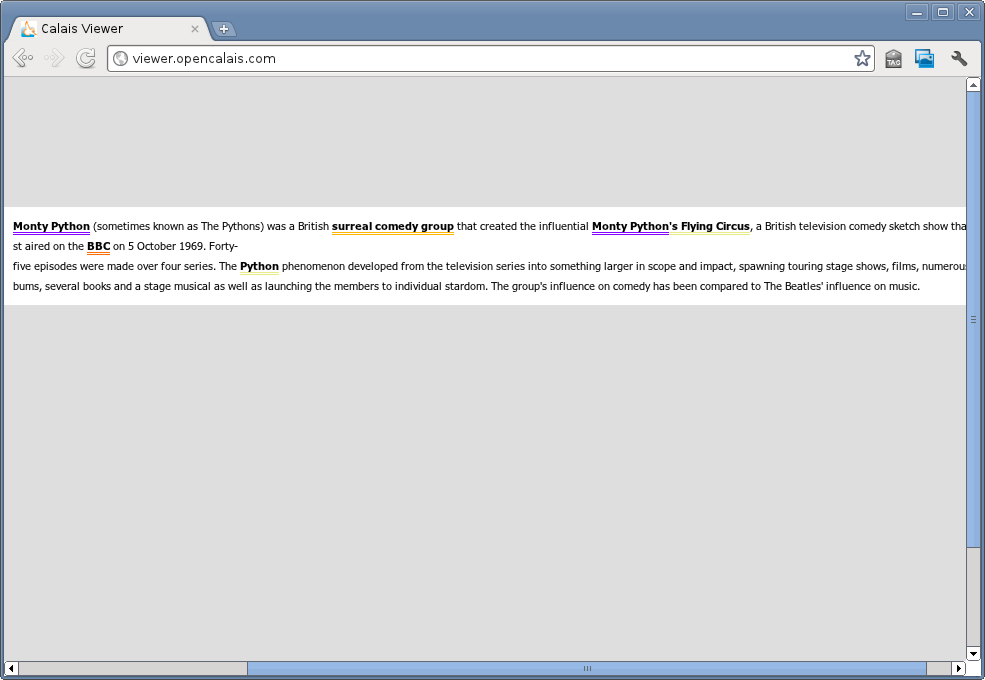
\includegraphics[width=.8\paperheight]{Analogs/CalaisViewer.png}
  \caption{Пример использования Web-приложения Calais Viewer}
  \label{fig:Analogs:OpenCalais}
\end{figure}
\end{landscape}

Функционирование системы OpenCalais основано на методах обработки
естественного языка, машинного обучения и других алгоритмах.

Для извлечения семантических метаданных применяются предварительно
подготовленные онтологии различных предметных областей в формате RDF.
Исходный текст подвергается предварительной обработке
(графематической и морфологической разметке), затем размеченные
словосочетания проходят идентификацию при помощи обученной модели
распознавания именованных сущностей, между которыми ведётся поиск
семантических отношений. Полученный граф сущностей и отношений между
ними преобразуется в набор RDF-троек.

Web-сервис OpenCalais бесплатен и доступен для некоммерческого и
коммерческого использования, однако требует регистрации для получения
API-ключа. Сервис построен по архитектуре REST \cite{Fielding00} и
использует формат XML \cite{XML} для обмена данными с пользователями.

На сегодняшний день, Web-сервис OpenCalais не способен обрабатывать
русскоязычные тексты.

\subsection{Extractor}
\label{subsec:Extractor}
Extractor — система автоматического извлечения терминов,
функционирующая с 2002 года и используемая многими организациями в
собственных решениях по обработке естественного языка
\cite{Extractor}.

Работа системы Extractor основана на применении генетических
алгоритмов \cite{Brownlee11} в сочетании с методами машинного
обучения и статистическими методами обработки естественного
языка \cite{Turney00}. Первоначальное обучение системы ведётся
на основе размеченного корпуса текстов.

Ознакомиться с возможностями Extractor можно при помощи
демонстрационного Web-приложения \url{ExtractorLive.com}.
Для создания собственных решений на основе технологии Extractor
необходимо приобрести набор инструментов разработчика. Пример
использования \url{ExtractorLive.com} приведён на
рисунке~\ref{fig:Analogs:Extractor}. Под заголовком “Keyphrases”
выведен список терминов, извлечённых из исходного текста, а под
заголовком “Highlights” показан результат автореферирования
исходного текста.

На сегодняшний день, Extractor не способен обрабатывать
русскоязычные тексты.

\begin{landscape}
\begin{figure}[ht]
  \centering
  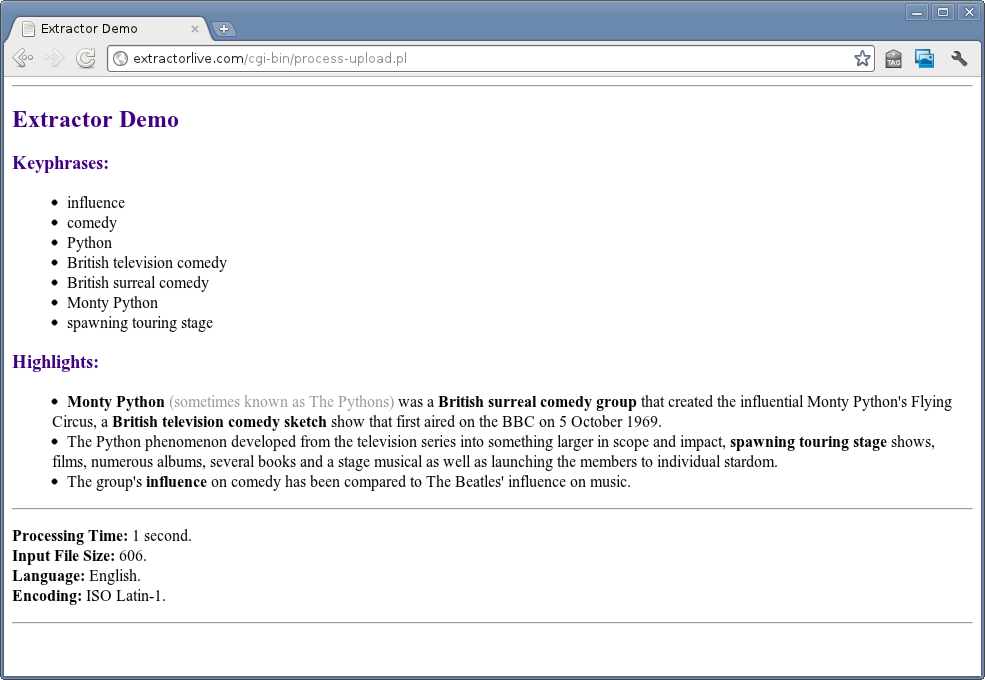
\includegraphics[width=.8\paperheight]{Analogs/ExtractorLive.png}
  \caption{Пример использования Web-приложения \url{ExtractorLive.com}}
  \label{fig:Analogs:Extractor}
\end{figure}
\end{landscape}

\subsection{Yahoo! Term Extraction Web Service}
\label{subsec:YahooTermExtractionWebService}
Yahoo! Term Extraction Web Service — сервис, используемый в поисковой
системе Yahoo! Search, предназначенный для извлечения ключевых фраз
из текста на естественном языке \cite{YahooTermExtractionWebService}.

Документация Yahoo! Term Extraction Web Service не упоминает
используемую технологию извлечения терминов.

Программный интерфейс Yahoo! Term Extraction Web Service доступен
наряду с другими сервисами в составе системы YQL. Обмен данными
с пользователем осуществляется в популярных форматах XML и JSON.

В данный момент, обработка русскоязычных текстов при помощи
Yahoo! Term Extraction Web Service невозможна.

Пример использования системы приведён на
рисунке~\ref{fig:Analogs:YahooTermExtractionWebService}. Результат
работы Yahoo! Term Extraction Web Service представлен в виде
XML-дерева и показан на вкладке “Tree” в виде списка кандидатов в
термины.

\begin{landscape}
\begin{figure}[ht]
  \centering
  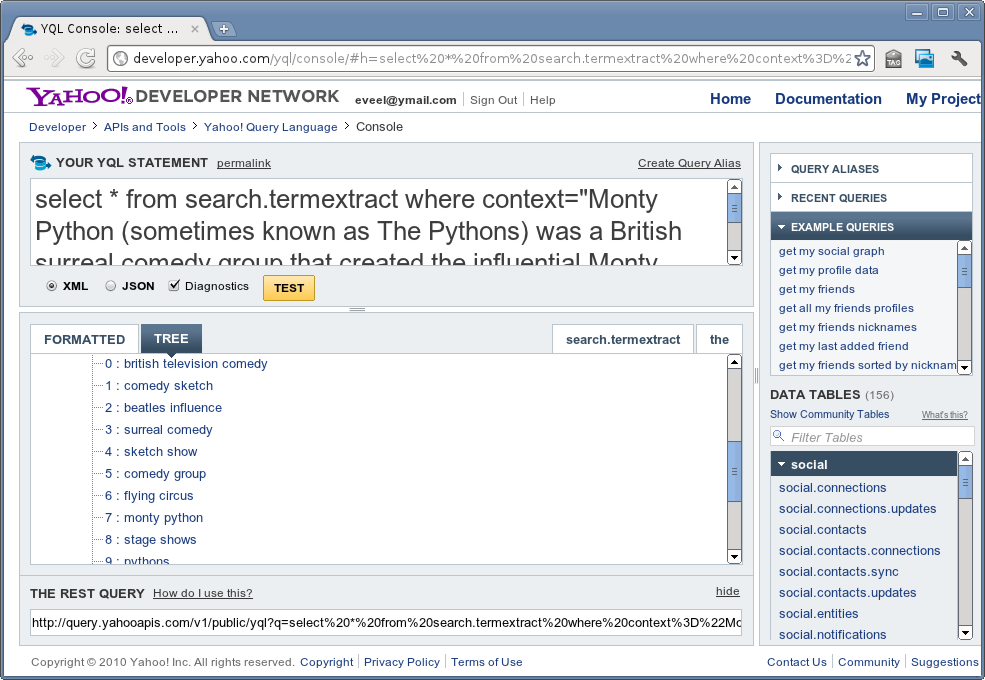
\includegraphics[width=.8\paperheight]{Analogs/YahooTermExtractionWebService.png}
  \caption{Пример запроса к Yahoo! Term Extraction Web Service
из консоли YQL}
  \label{fig:Analogs:YahooTermExtractionWebService}
\end{figure}
\end{landscape}

\subsection{TerMine}
\label{subsec:TerMine}
TerMine — Web-сервис извлечения терминов, разработанный в
британском Национальном центре анализа текста (англ.
\emph{The National Centre for Text Mining}) \cite{TerMine}.

Сервис TerMine работает на основе метода C-value, описанного в
\cite{Frantzi00} и применяет анализатор TreeTagger \cite{TreeTagger}
для предварительной морфологической разметки текста.

Демонстрационный Web-интерфейс TerMine позволяет обрабатывать
тексты объёмом до 2 мегабайт исключительно на английском языке.

Пример использования системы приведён на
рисунке~\ref{fig:Analogs:TerMine}: термины, извлечённые из исходного
текста, выделены красным цветом.

\begin{landscape}
\begin{figure}[ht]
  \centering
  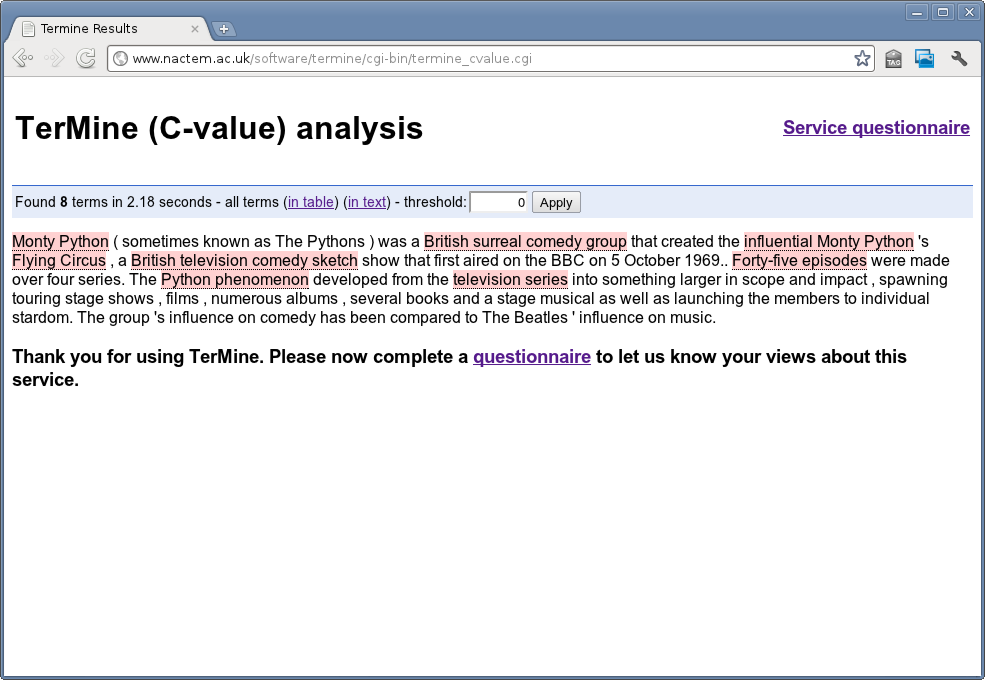
\includegraphics[width=.8\paperheight]{Analogs/TerMine.png}
  \caption{Пример использования демонстрационного Web-интерфейса
TerMine}
  \label{fig:Analogs:TerMine}
\end{figure}
\end{landscape}

\subsection{Maui}
\label{subsec:Maui}
Maui — система тематической классификации текстовых документов,
работающая на основе методов обработки естественного языка и
машинного обучения \cite{Medelyan09}. Схема функционирования
системы приведена состоит из двух этапов работы: этапа
первоначального построения и обучения модели, и этапа
применения обученной модели к решению задачи тематической
классификации текста.

Результаты тематической классификации, полученные при помощи Maui,
могут рассматриваться в качестве тегов (меток) исходного текста.
Без использования обученной модели, Maui функционирует как система
автоматического извлечения ключевых фраз (в данной работе оценка
системы Maui проводилась без использования обученной модели).

Система Maui является свободным кроссплатформенным программным
обеспечением и распространяется на условиях лицензии GNU General
Public License Version 3. При помощи Web-приложения maui-indexer
\cite{Maui} можно ознакомиться с основными возможностями системы
(рисунок~\ref{fig:Analogs:Maui}). В этом случае, ключевые слова и
фразы перечислены в блоке “Keywords”.

В настоящий момент, Maui не способна обрабатывать русскоязычные
тексты.

\begin{landscape}
\begin{figure}[ht]
  \centering
  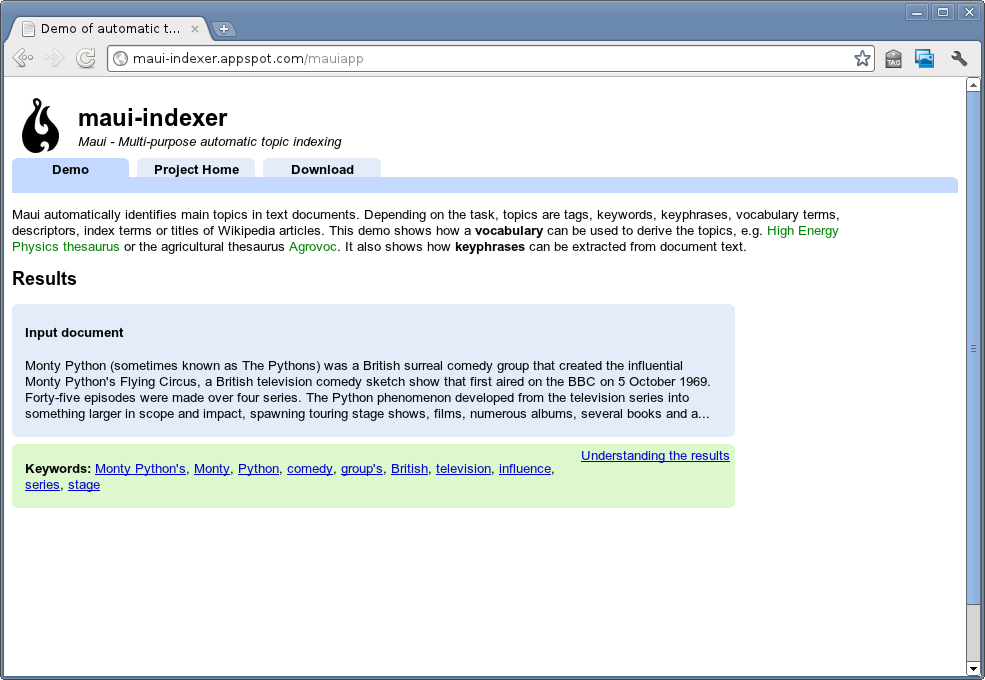
\includegraphics[width=.8\paperheight]{Analogs/MauiIndexer.png}
  \caption{Пример использования Web-приложения maui-indexer}
  \label{fig:Analogs:Maui}
\end{figure}
\end{landscape}

\subsection{TextAnalyst}
\label{subsec:TextAnalyst}
TextAnalyst — инструмент для смыслового поиска информации и анализа
содержания текстов \cite{TextAnalyst}, имеющий возможность выделения
ключевых слов. Функционирование TextAnalyst основано на применении
методов обработки естественного языка в сочетании с методами
машинного обучения.

Пакет TextAnalyst доступен для ознакомительного использования в
виде приложения для семейства операционных систем
Microsoft\textregistered~Windows\textregistered и способен
обрабатывать тексты на русском языке.

Пример использования TextAnalyst приведён на
рисунке~\ref{fig:Analogs:TextAnalyst}. Ключевые слова исходного
текста ключевые слова выделены зелёным цветом.

\begin{landscape}
\begin{figure}[ht]
  \centering
  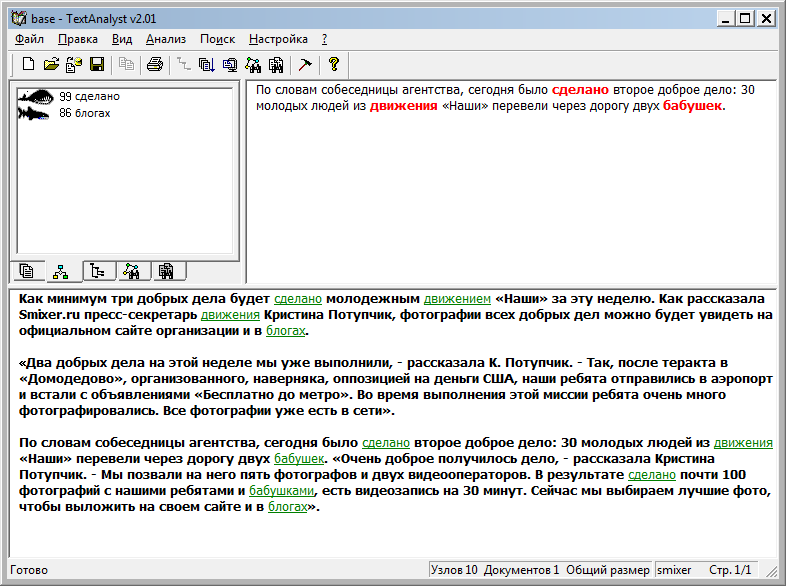
\includegraphics[width=.7\paperheight]{Analogs/TextAnalyst.png}
  \caption{Пример использования пакета TextAnalyst}
  \label{fig:Analogs:TextAnalyst}
\end{figure}
\end{landscape}

\subsection{АОТ}
\label{subsec:AOT}
АОТ — проект, направленный на создание системы автоматического
перевода «ДИАЛИНГ» \cite{AOT}. В рамках проекта АОТ разработан
комплекс инструментов автоматической обработки текста, в том числе
графематический, морфологический и синтаксический анализаторы
русского языка.

Все инструменты, разработанные в рамках проекта АОТ (в том числе и
синтаксический анализатор) являются свободным кроссплатформенным
программным обеспечением и распространяются на условиях лицензии
GNU Lesser General Public License Version 2.1.

Пример использования анализатора приведён на
рисунке~\ref{fig:Analogs:AOT}. Именные группы, выделенные при помощи
анализатора AOT, можно принять в качестве терминов--кандидатов
исходного текста \cite{Braslavsky08}.

\begin{landscape}
\begin{figure}[ht]
  \centering
  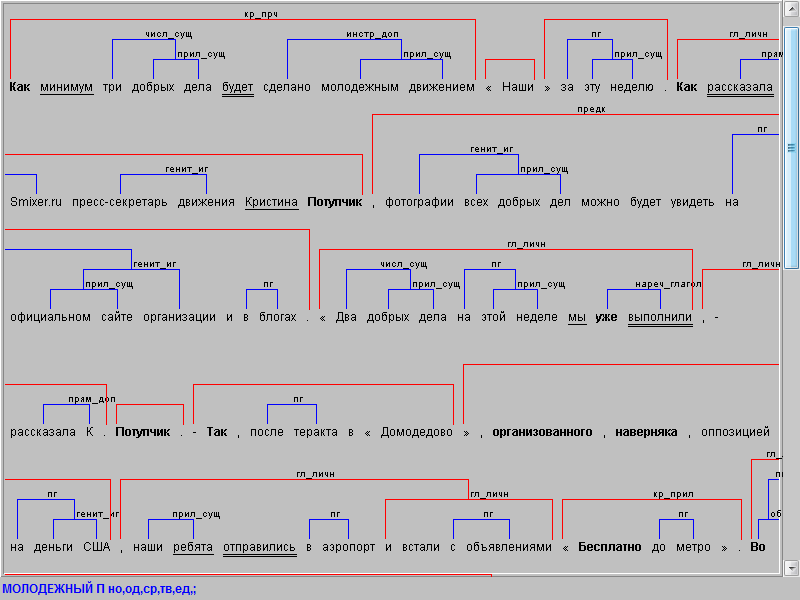
\includegraphics[width=.7\paperheight]{Analogs/AOT.png}
  \caption{Пример использования синтаксического анализатора АОТ}
  \label{fig:Analogs:AOT}
\end{figure}
\end{landscape}

\subsection{ContentAnalyzer}
\label{subsec:ContentAnalyzer}
ContentAnalyzer — инструмент для анализа содержания тематических
Web-страниц в реальном времени, выделения списков ключевых слов и
словосочетаний, построения автореферата текста документа
\cite{ContentAnalyzer}.

Функционирование ContentAnalyzer обеспечивается за счёт вычисления
таких характеристик текста, как:
\begin{itemize}
  \item частота термина/словосочетания в документе;
  \item отношение частоты к числу слов документа;
  \item вес термина в документе (с учётом частоты и весовых
коэффициентов);
  \item вес термина к числу слов документа, и\ др.
\end{itemize}

Пакет ContentAnalyzer распространяется бесплатно, доступен для
использования в виде приложения для семейства операционных систем
Microsoft\textregistered~Windows\textregistered
и способен обрабатывать тексты как на русском, так и на
английском языках.

Пример использования ContentAnalyzer приведён на
рисунке~\ref{fig:Analogs:ContentAnalyzer}: пакет рассчитал
заявленные характеристики текста, выполнил извлечение ключевых
слов и фраз, а также провёл автореферирование текста.

\begin{landscape}
\begin{figure}[ht]
  \centering
  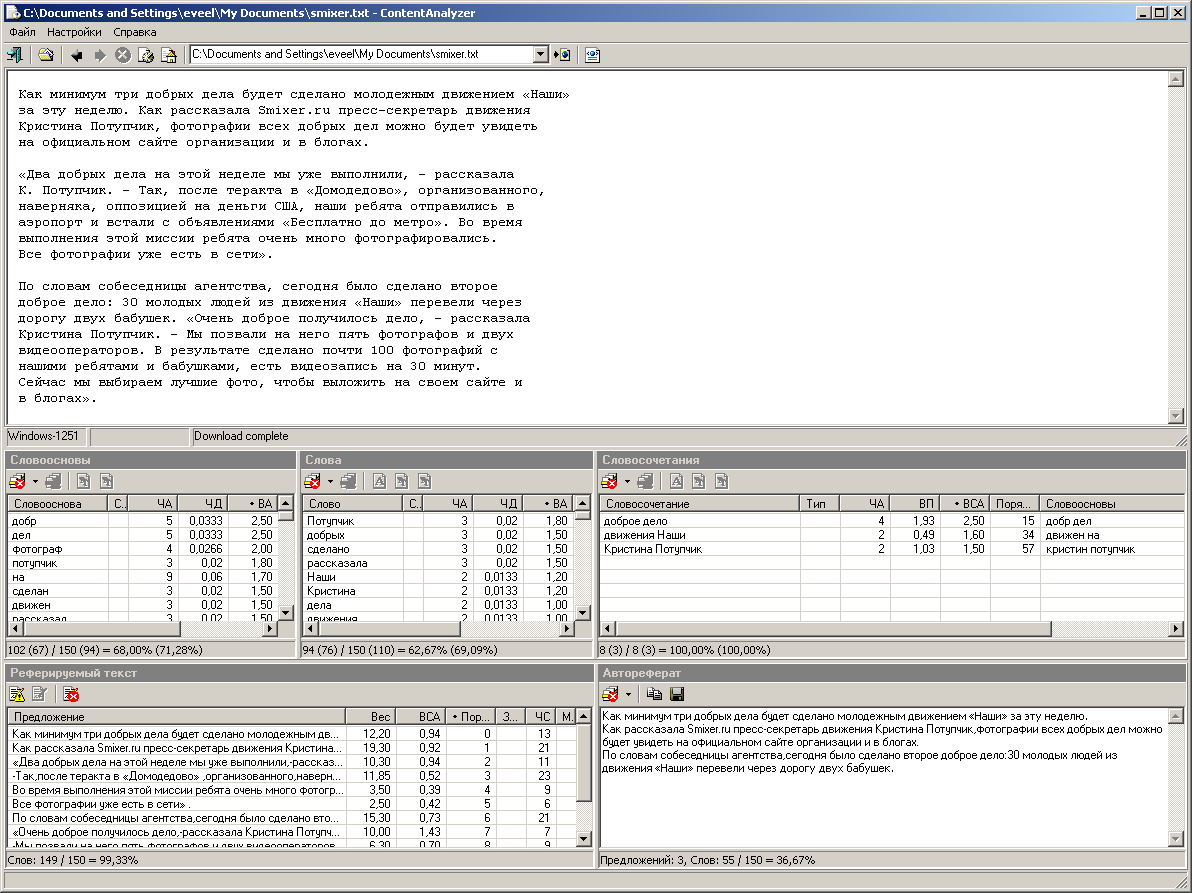
\includegraphics[width=.7\paperheight]{Analogs/ContentAnalyzer.png}
  \caption{Пример использования ContentAnalyzer}
  \label{fig:Analogs:ContentAnalyzer}
\end{figure}
\end{landscape}

\subsection{Семантическое зеркало}
\label{subsec:SemanticMirror}
Семантическое зеркало — система тематической классификации
Web-страниц \cite{SemanticMirror}, разработанная компанией
«Ашманов и партнёры».

Сервис «Семантическое зеркало» обрабатывает текст Web-страницы и
определяет её тему: анализирует слова, семантические связи между
ними, выделяет самые важные термины. Темы определяются по
рубрикатору, где к каждой рубрике приписано некоторое множество
терминов.

Результат тематической классификации можно использовать в качестве
списка ключевых фраз исходного текста или в качестве набора тегов
(меток). Эту информацию можно использовать для показа контекстной
рекламы и новостей на актуальную тему.

На сайте компании «Ашманов и партнёры» доступна демонстрационная
версия «Семантического зеркала», имеющая лимит в 128 обращений с
одного IP-адреса в сутки. Сервис обрабатывает тексты как на русском,
так и на английском языках.

Пример использования сервиса приведён на
рисунке~\ref{fig:Analogs:SemanticMirror}: для каждого
термина--кандидата вычислен его вес в исходном тексте. На основании
этих данных корректно определена тема документа.

\begin{landscape}
\begin{figure}[ht]
  \centering
  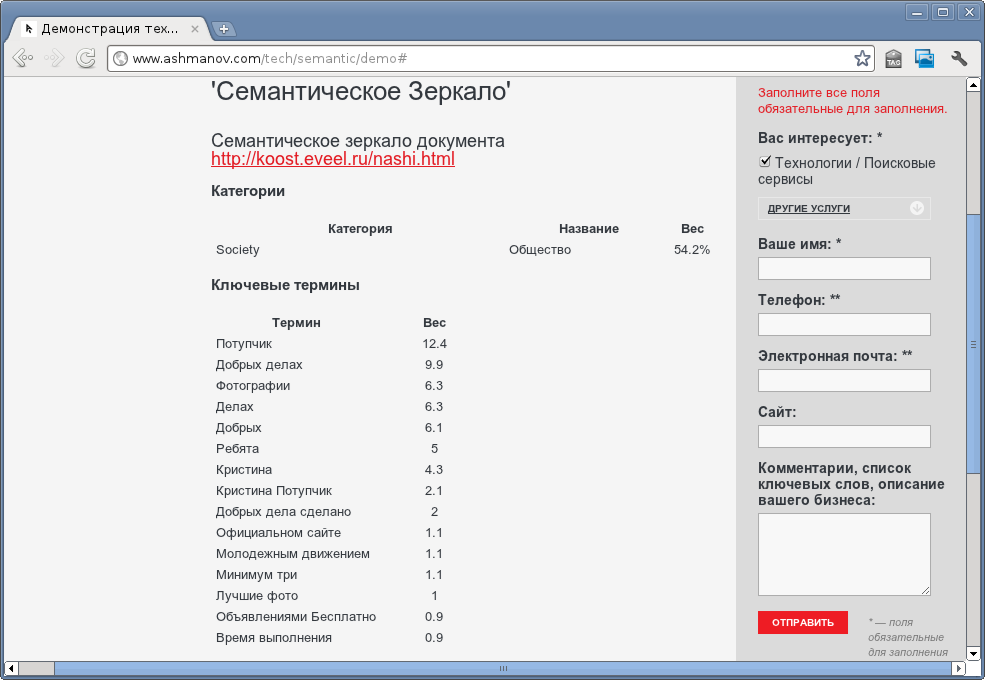
\includegraphics[width=.8\paperheight]{Analogs/SemanticMirror.png}
  \caption{Пример использования сервиса «Семантическое зеркало»}
  \label{fig:Analogs:SemanticMirror}
\end{figure}
\end{landscape}

\section{Формирование набора критериев}
\label{sec:Criteria}
Необходимая система автоматического извлечения ключевых фраз из текста
на естественном языке оценивается по следующим практически
важным критериям:
\begin{itemize}
  \item поддержка русского языка (``Р''):
  \begin{itemize}
    \item 0.0 — поддержка отсутствует;
    \item 1.0 — поддержка присутствует.
  \end{itemize}
  \item качество результата по итогам экспертной оценки (``К''):
  \begin{itemize}
    \item 0.0 — минимальная оценка;
    \item 1.0 — максимальная оценка.
  \end{itemize}
  \item доступность аналога (``Д''):
  \begin{itemize}
    \item 0.0 — использование аналога требует приобретения платной
лицензии или временной подписки;
    \item 0.5 — существуют полноценные бесплатные версии аналога,
$\beta$-версии или специальные версии для академических исследований;
    \item 1.0 — аналог распространяется как
свободное программное обеспечение.
  \end{itemize}
  \item независимость аналога от наличия онтологии заданной
области знаний или специализированного тезауруса в процессе
извлечения ключевых фраз (``О''):
  \begin{itemize}
    \item 0.0 — аналог спроектирован с целью использования
специализированного тезауруса или онтологии области знаний
в процессе выделения терминов;
    \item 1.0 — результат выделения терминов не зависит от
наличия специализированного тезауруса или онтологии области
знаний.
  \end{itemize}
\end{itemize}

\section{Сравнение аналогов}
В результате обзора современных систем извлечения ключевых
фраз из текста на естественном было найдено 9 аналогов.
Для того, чтобы перейти к выбору прототипа, необходимо оценить
каждый из аналогов в соответствии с критериями, обозначенными
в \ref{sec:Criteria}.

Составим таблицу~\ref{tab:Analogs}, в которой оценим
аналоги по качественному уровню проявления критериев,
выбранных в \ref{sec:Criteria}.

\begin{table}[H]
\caption{\label{tab:Analogs}Сравнение существующих
аналогов по заданным критериям.}
\begin{tabular}{|c||c||*{4}{p{1cm}|}|c|}
\hline
  & Название & \multicolumn{4}{c||}{Оценки по критериям} & \\
                \cline{3-6}
№ & аналога         &  Р  &  К  &  Д  &  О  & \huge $\Sigma$ \\
\hline
\hline
1 & OpenCalais      & 0.0 & 0.8 & 0.5 & 0.0 & 1.3 \\
\hline
2 & Extractor       & 0.0 & 0.7 & 0.0 & 1.0 & 1.7 \\
\hline
3 & Yahoo! Term Extraction Web Service
                    & 0.0 & 0.6 & 0.5 & 1.0 & 2.1 \\
\hline
4 & TerMine         & 0.0 & 0.7 & 0.5 & 1.0 & 2.2 \\
\hline
5 & Maui            & 0.0 & 0.6 & 1.0 & 1.0 & 2.6 \\
\hline
6 & TextAnalyst     & 1.0 & 0.3 & 0.5 & 1.0 & 2.8 \\
\hline
\textbf{7} & \textbf{AOT}
                    & 1.0 & 0.4 & 1.0 & 1.0 & \textbf{3.4} \\
\hline
8 & ContentAnalyzer & 1.0 & 0.6 & 0.5 & 1.0 & 3.1 \\
\hline
9 & Семантическое
     зеркало        & 1.0 & 0.5 & 0.5 & 1.0 & 3.0 \\
\hline
\end{tabular}
\end{table}

\section{Работа с прототипами}
В результате попарного сравнения аналогов (таблица~\ref{tab:Analogs})
по заданным критериям \ref{sec:Criteria}, целесообразным оказывается
выбор аналога №7 (АОТ, выделено жирным) в качестве прототипа системы
автоматического извлечения ключевых фраз из текста на
естественном языке.

Структурная и алгоритмическая модели прототипа представлены на
рисунках~\ref{fig:Prototype} и \ref{fig:Prototype-Algorithm}.

\begin{figure}[ht]
  \centering
  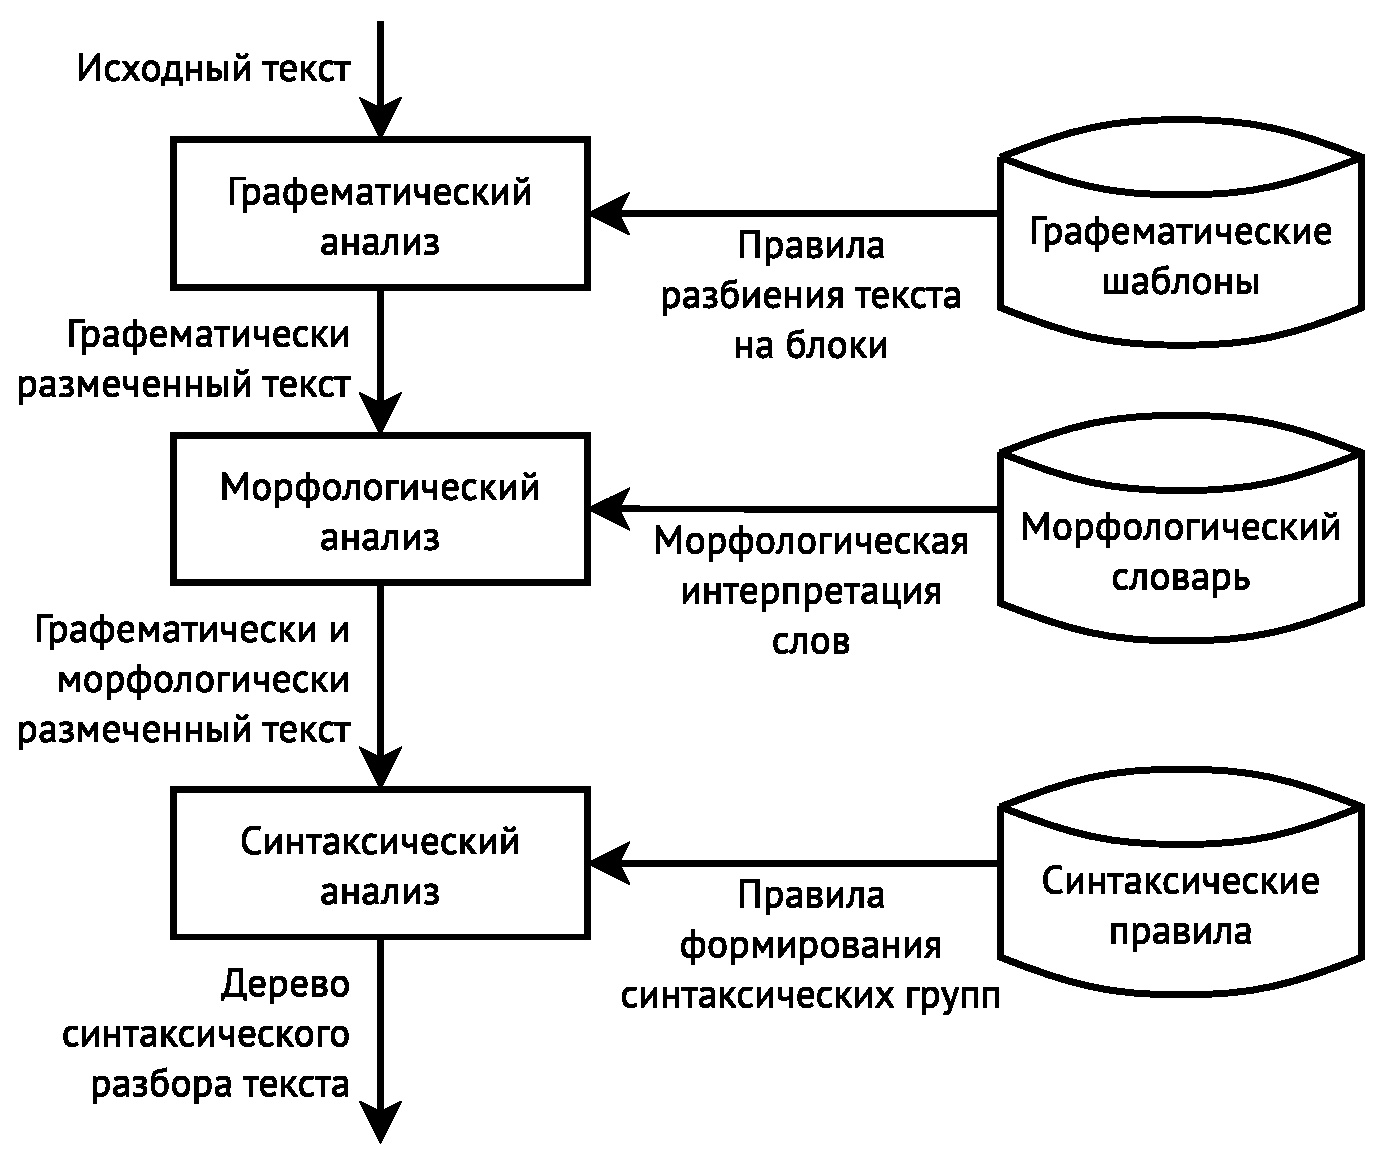
\includegraphics[scale=0.5]{Prototype.eps}
  \caption{Структурная модель прототипа системы автоматического
извлечения ключевых фраз из текста на естественном языке}
  \label{fig:Prototype}
\end{figure}

\begin{figure}[ht]
  \centering
  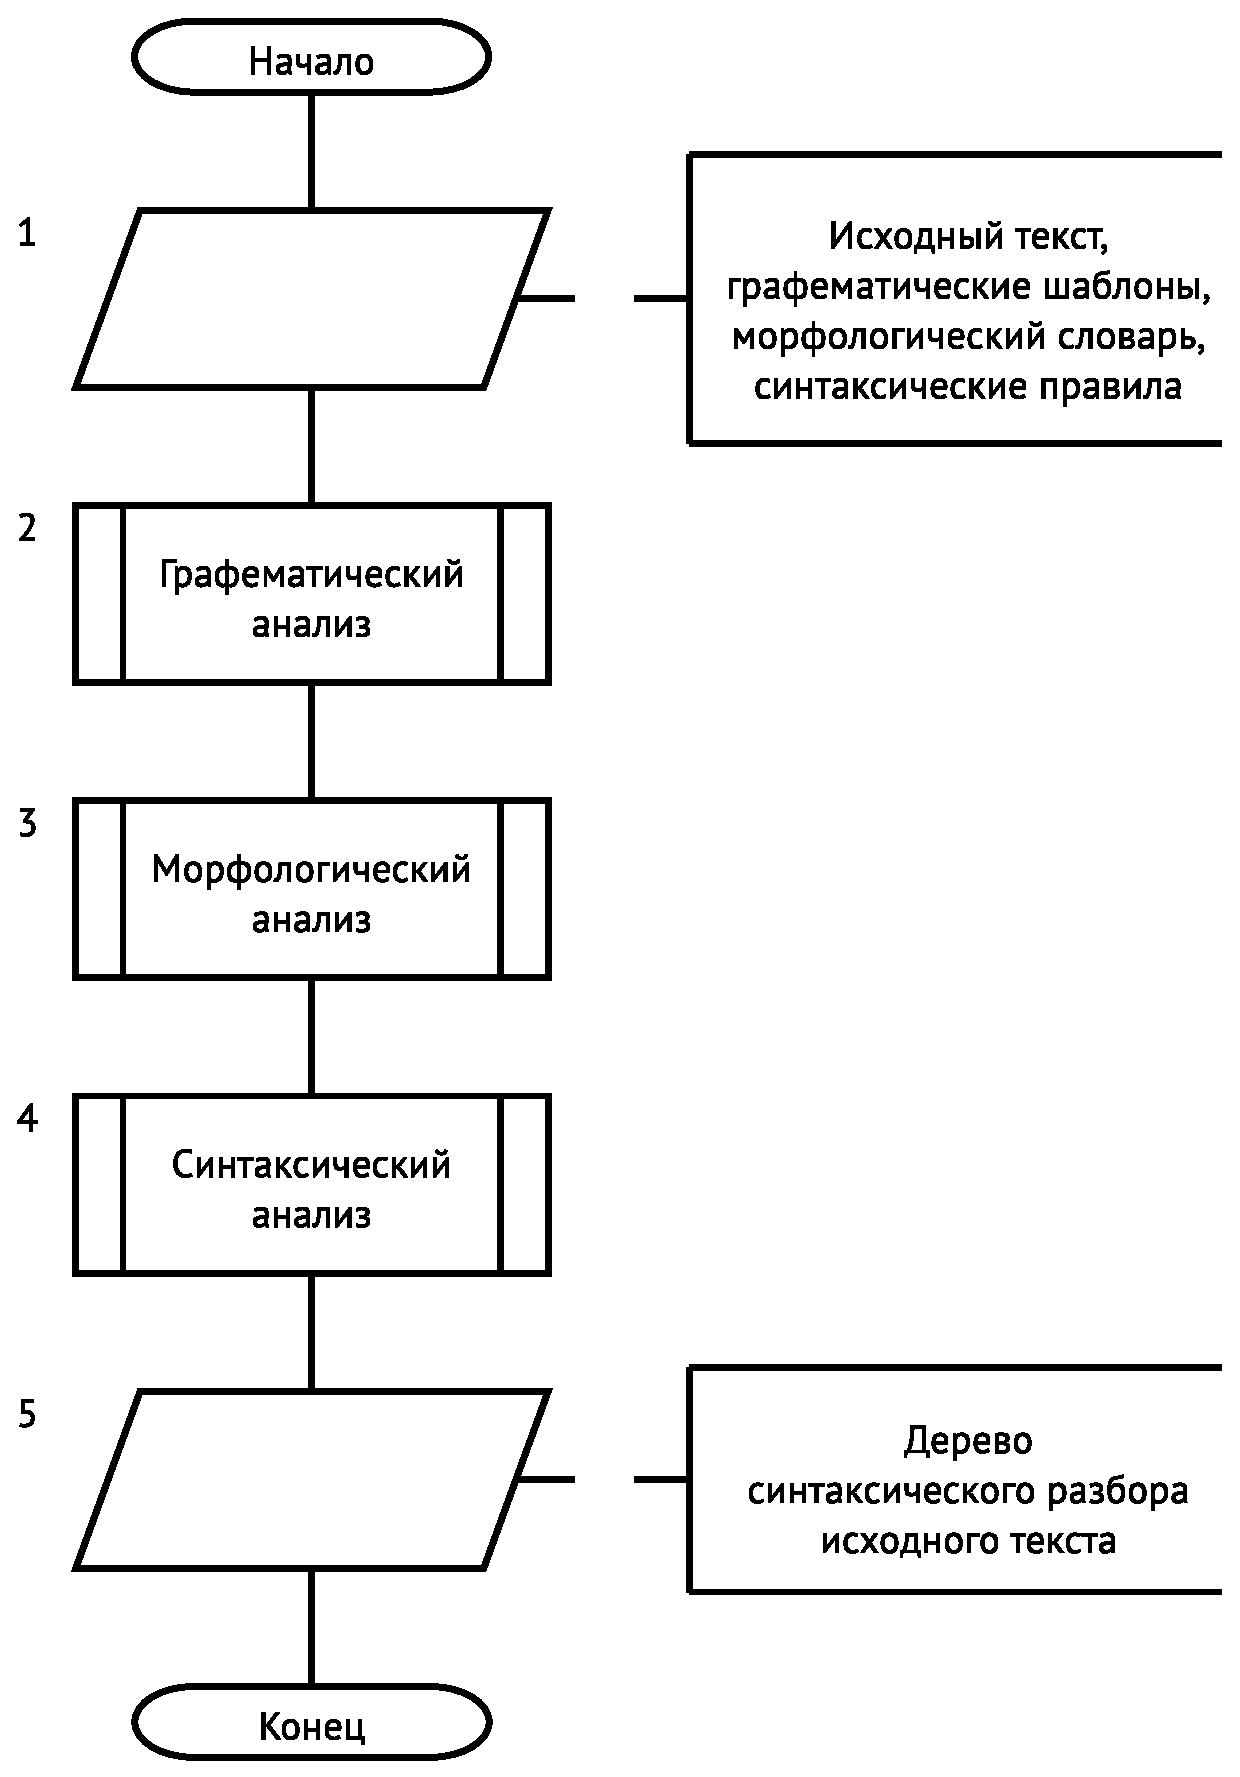
\includegraphics[scale=0.5]{Prototype-Algorithm.eps}
  \caption{Алгоритмическая модель прототипа системы автоматического
извлечения ключевых фраз из текста на естественном языке}
  \label{fig:Prototype-Algorithm}
\end{figure}

Компоненты, составляющие языковую модель
(рисунок~\ref{fig:Prototype}), — лингвистические процессоры,
которые друг за другом обрабатывают входной текст. Вход одного
процессора является выходом другого. Выделяются следующие
компоненты:
\begin{itemize}
  \item графематический анализатор;
  \item морфологический анализатор;
  \item синтаксический анализатор.
\end{itemize}

Графематический анализ — это начальный этап анализа
естественноязыкового текста, представленного в виде цепочки символов
\cite{AOTGraphAn}. На этом этапе вырабатывается информация, необходимая
для дальнейшей обработки морфологическим и синтаксическим анализаторами.
В задачу графематического анализа входят: разделение входного текста на
слова и разделители; выделение предложений из входного текста; выделение
абзацев, заголовков, примечаний, и\ др. Подробное описание принципа
функционирования графематического анализатора АОТ приведено в
\cite{AOTGraphAn}.

Задача морфологического анализатора — построение морфологической
интерпретации слов входного текста \cite{Nozhov03}. Подробное описание
морфологического анализатора АОТ приведено в \cite{Sokirko04}.
Для каждого слова входного текста выдается множество морфологических
интерпретаций следующего вида:
\begin{itemize}
  \item морфологическая часть речи (например, род, число, падеж,
и\ т.\ д.)
  \item лемма — каноническая форма лексемы (например, существительное в
именительном падеже единственного числа, или глагол--инфинитив);
  \item множество наборов граммем — элементарных описателей, относящих
словоформу к какому--либо морфологическому классу.
\end{itemize}

Цель синтаксического анализа — построение дерева зависимостей
каждого предложения входного текста. Дерево представлено в виде
ориентированного графа, вершинами которого являются синтаксические
группы \cite{Levine06}, построенные из слов входного текста,
а дугами являются отношения между синтаксическими группами
\cite{Nozhov03}. Группы строятся при помощи заранее определённых
синтаксических правил \cite{Gladky85}. Описание алгоритма
синтаксического анализа АОТ приведено в \cite{Nozhov03}.

Известно, что большинство терминов – это именные группы, что
позволяет в качестве терминов--кандидатов рассматривать именные
группы, выделенные с помощью синтаксического анализатора
\cite{Braslavsky08}. На рисунке~\ref{fig:Analogs:AOT} видно,
что на основе слов входного текста получена древовидная
структура, содержащая различные синтаксические группы. Среди
всех возможных групп, особый интерес для нашей задачи представляют
именные группы (обозначены “прил\_сущ” и “генит\_иг”):
\begin{itemize}
  \item добрых дела;
  \item наши ребята;
  \item пресс--секретарь движения;
  \item и\ т.\ д.
\end{itemize}

Описание схемы функционирования прототипа наглядно представлено на
рисунке~\ref{fig:Example} с учётом прохождения всех описанных
уровней обработки текста, начиная с графематического анализа,
заканчивая разбором предложений с формированием синтаксических групп.

\begin{figure}[!ht]
  \centering
  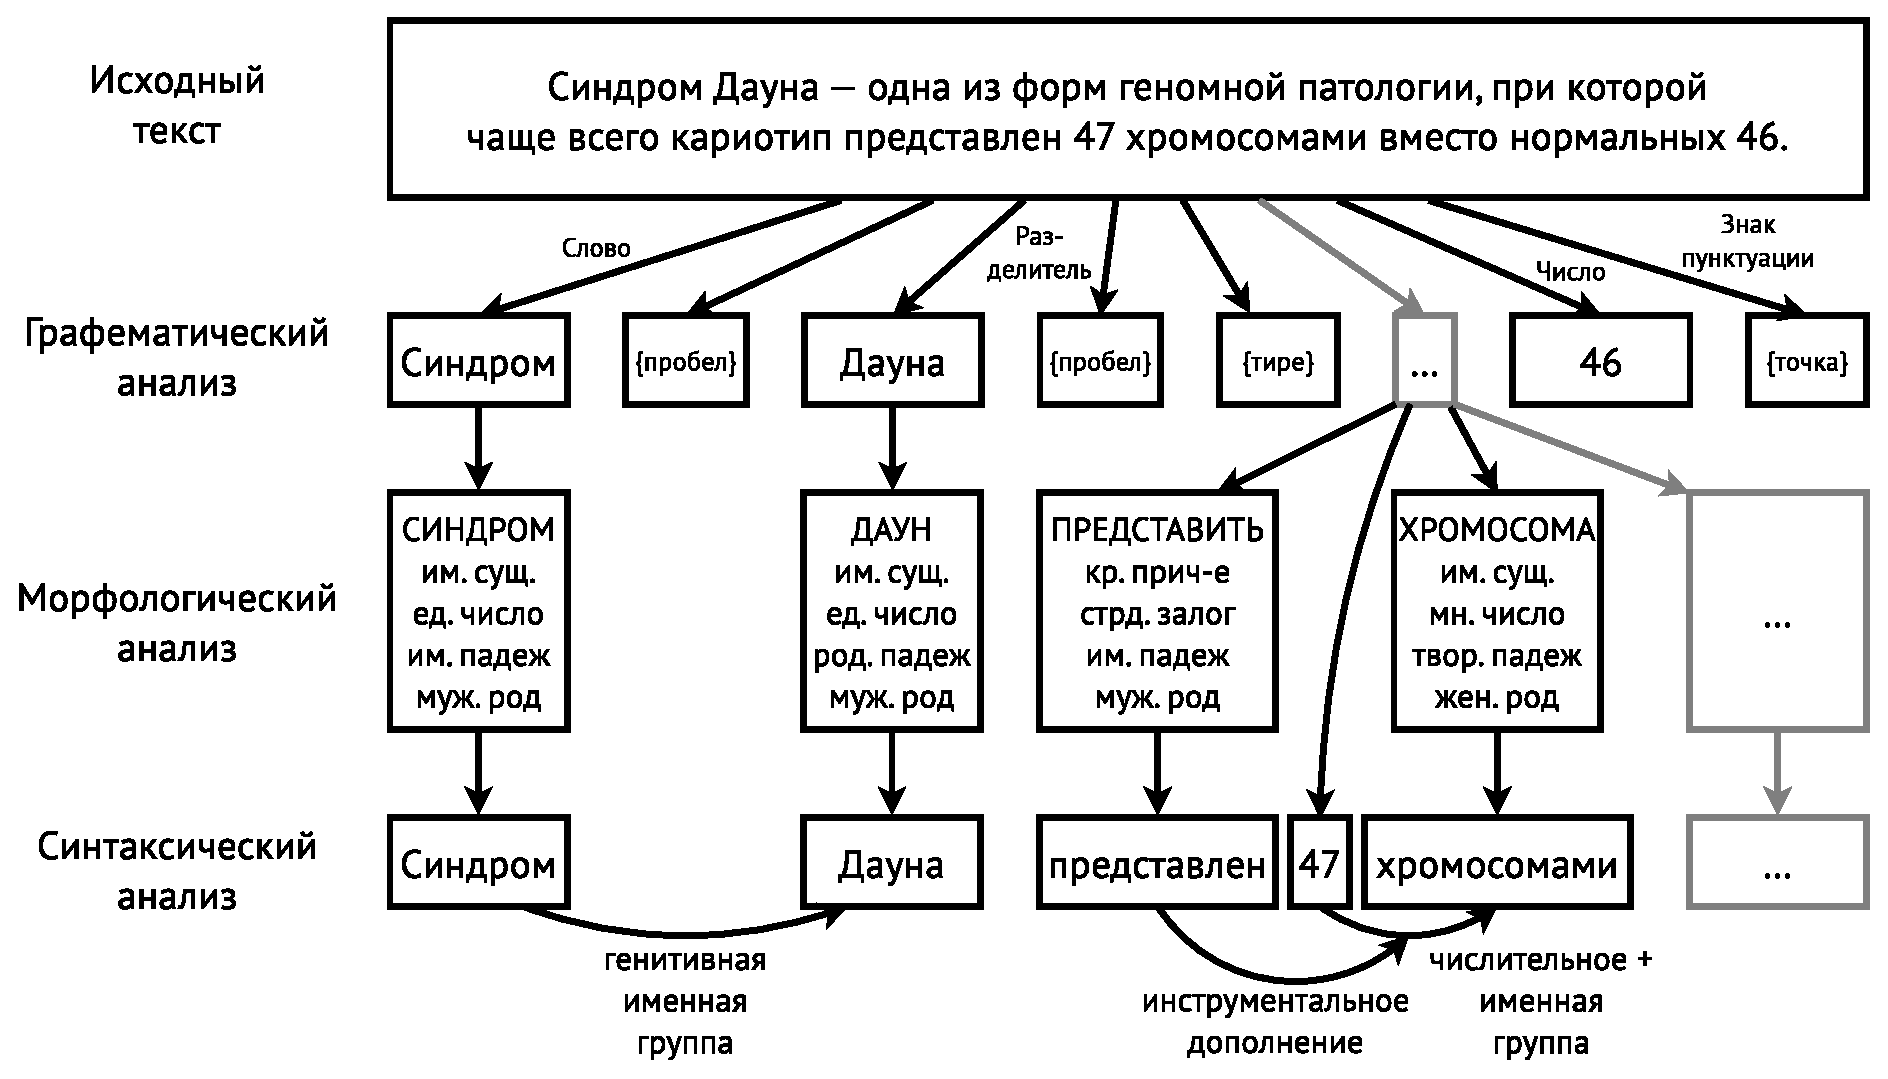
\includegraphics[scale=0.5]{Example.eps}
  \caption{Пример работы прототипа}
  \label{fig:Example}
\end{figure}

\subsection{Критика прототипа}
\label{subsec:Critic}
Из структуры выбранного прототипа (рисунок~\ref{fig:Prototype}),
алгоритма его функционирования (рисунок~\ref{fig:Prototype-Algorithm})
и результатов его сравнения с существующими аналогами
(таблица~\ref{tab:Analogs}) по критериям \ref{sec:Criteria} очевидно,
что применённый в прототипе метод распознавания многословных терминов
обладает недостаточной точностью \cite{Braslavsky08}. Необходима его
доработка с целью явного определения ключевых слов и фраз, наиболее
адекватных исходному тексту, а также их ранжирования на основе
статистического значения терминологичности.

Кроме того, стоит отметить, что качество работы современных
морфологических анализаторов превосходит \cite{Lyashevskaya10}
морфологический анализатор АОТ \cite{Sokirko04}.

\subsection{Предлагаемое решение}
\label{subsec:Solution}
В целях повышения адекватности результата извлечения ключевых фраз
прототипом, предлагается внести в его структуру блок, вычисляющий
статистическое значение терминологичности каждой именной группы,
выделенной синтаксическим анализатором.

Из результатов попарного сравнения аналогов
(таблица~\ref{tab:Analogs}) видно, что аналог TerMine
(\ref{subsec:TerMine}) получил наивысшую оценку качества результата
работы среди систем, не использующих онтологию заданной области
знаний в процессе выделения терминов.

Подобно системе TerMine, стоит воспользоваться статистическим методом
C-value \cite{Frantzi00}, что позволит сопоставить каждой извлечённой из
текста именной группе значение терминологичности, вычисляемое по формуле:
\begin{equation}
  C-value(a) = \begin{cases}
    log_{2}|a| \cdot f(a), &
                 \mbox{если } a \mbox{ не вложен} \\
    log_{2}|a| \cdot f(a) - \frac{1}{P(T_{a})}
               \cdot \sum_{b \in T_{a}} f(b), &
                 \mbox{если } a \mbox{ вложен},
  \end{cases}
  \label{eq:CValue}
\end{equation}
где $a$ — кандидат в термины; \\
$|a|$ — длина словосочетания, измеряемая в количестве слов; \\
$f(a)$ — частотность $a$; \\
$T_{a}$ — множество словосочетаний, которые содержат $a$; \\
$P(T_{a})$ — количество словосочетаний, содержащих $a$.

Легко видеть, что чем больше частота встречаемости термина--кандидата
в тексте и чем выше его длина, тем больше его вес в исходном тексте.
Однако если этот кандидат входит в большое количество других
словосочетаний, то его вес уменьшается \cite{Frantzi00}. Путём
сортировки списка кандидатов в термины по убыванию значения C-value
можно получить список ключевых фраз, наиболее адекватных исходному
тексту \cite{Braslavsky08}.

Таким образом, в структуру прототипа, изображенную на
рисунке~\ref{fig:Prototype} целесообразно внести готовое решение
1-го ранга — блок явного выделения ключевых фраз на основе
метода C-value.

Структурная и алгоритмическая модели блока выделения ключевых
фраз (решения 1-го ранга) представлены на
рисунках~\ref{fig:Solution-Rank1a} и
\ref{fig:Solution-Algorithm-Rank1a}.

\begin{figure}[ht]
  \centering
  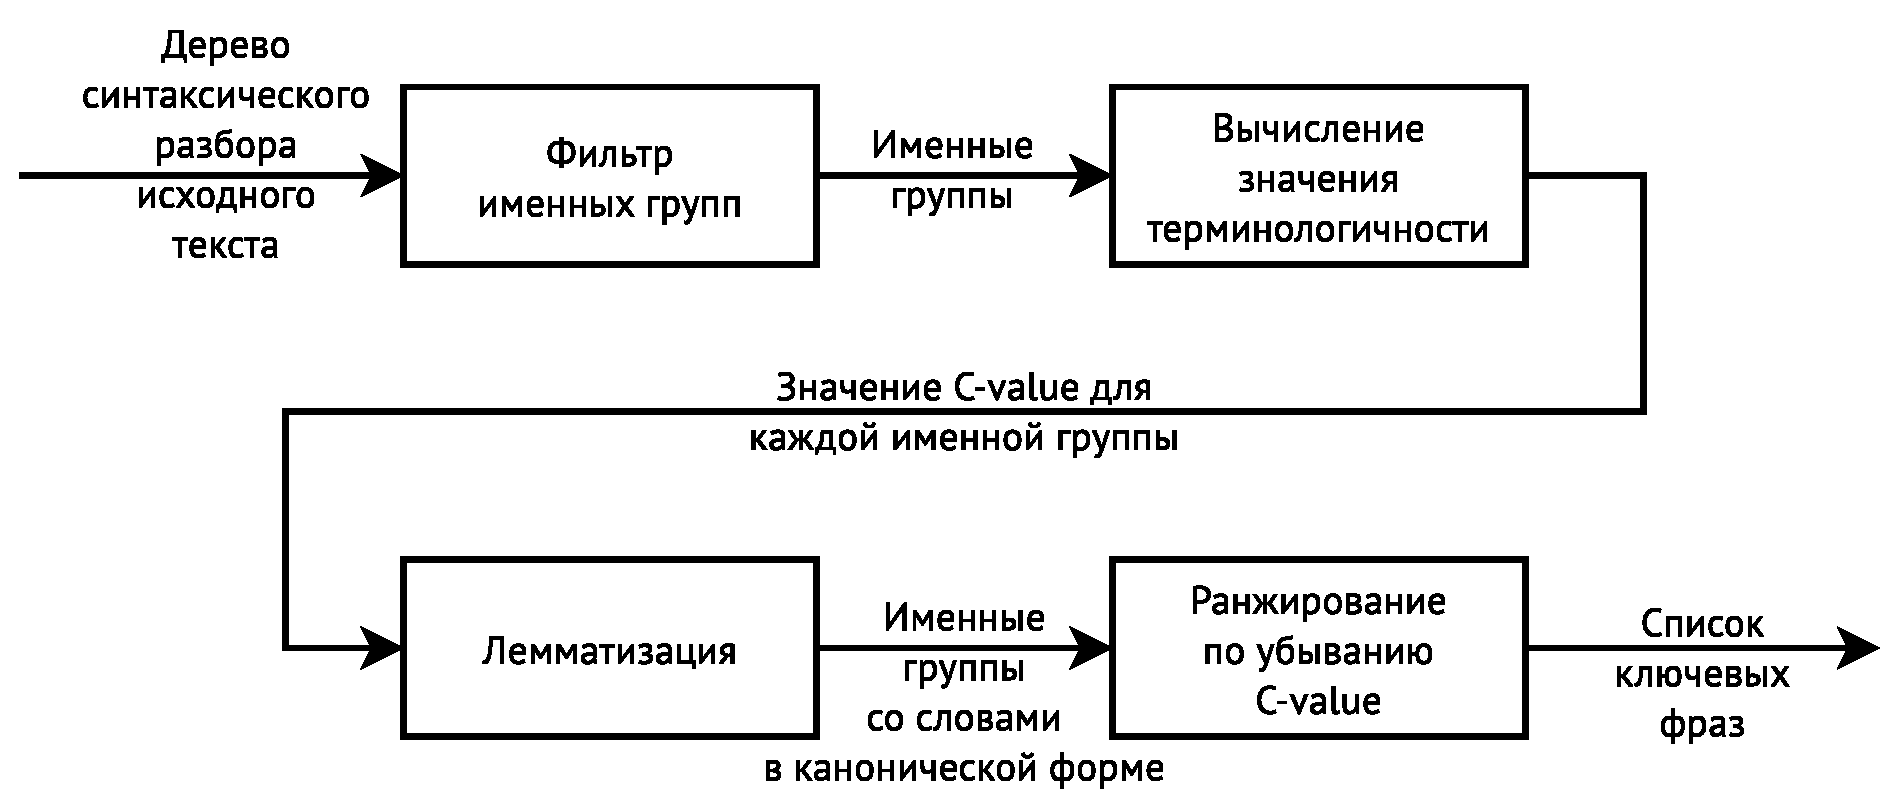
\includegraphics[scale=0.5]{Solution-Rank1a.eps}
  \caption{Структурная модель блока выделения ключевых фраз —
решения 1-го ранга}
  \label{fig:Solution-Rank1a}
\end{figure}

Также в качестве меры по повышению точности извлечения
ключевых фраз из текста, необходимо модифицировать морфологический
анализатор системы АОТ, что повысит качество предварительной
обработки текста и положительно скажется на результате работы
всей системы в целом.

\begin{figure}[H]
  \centering
  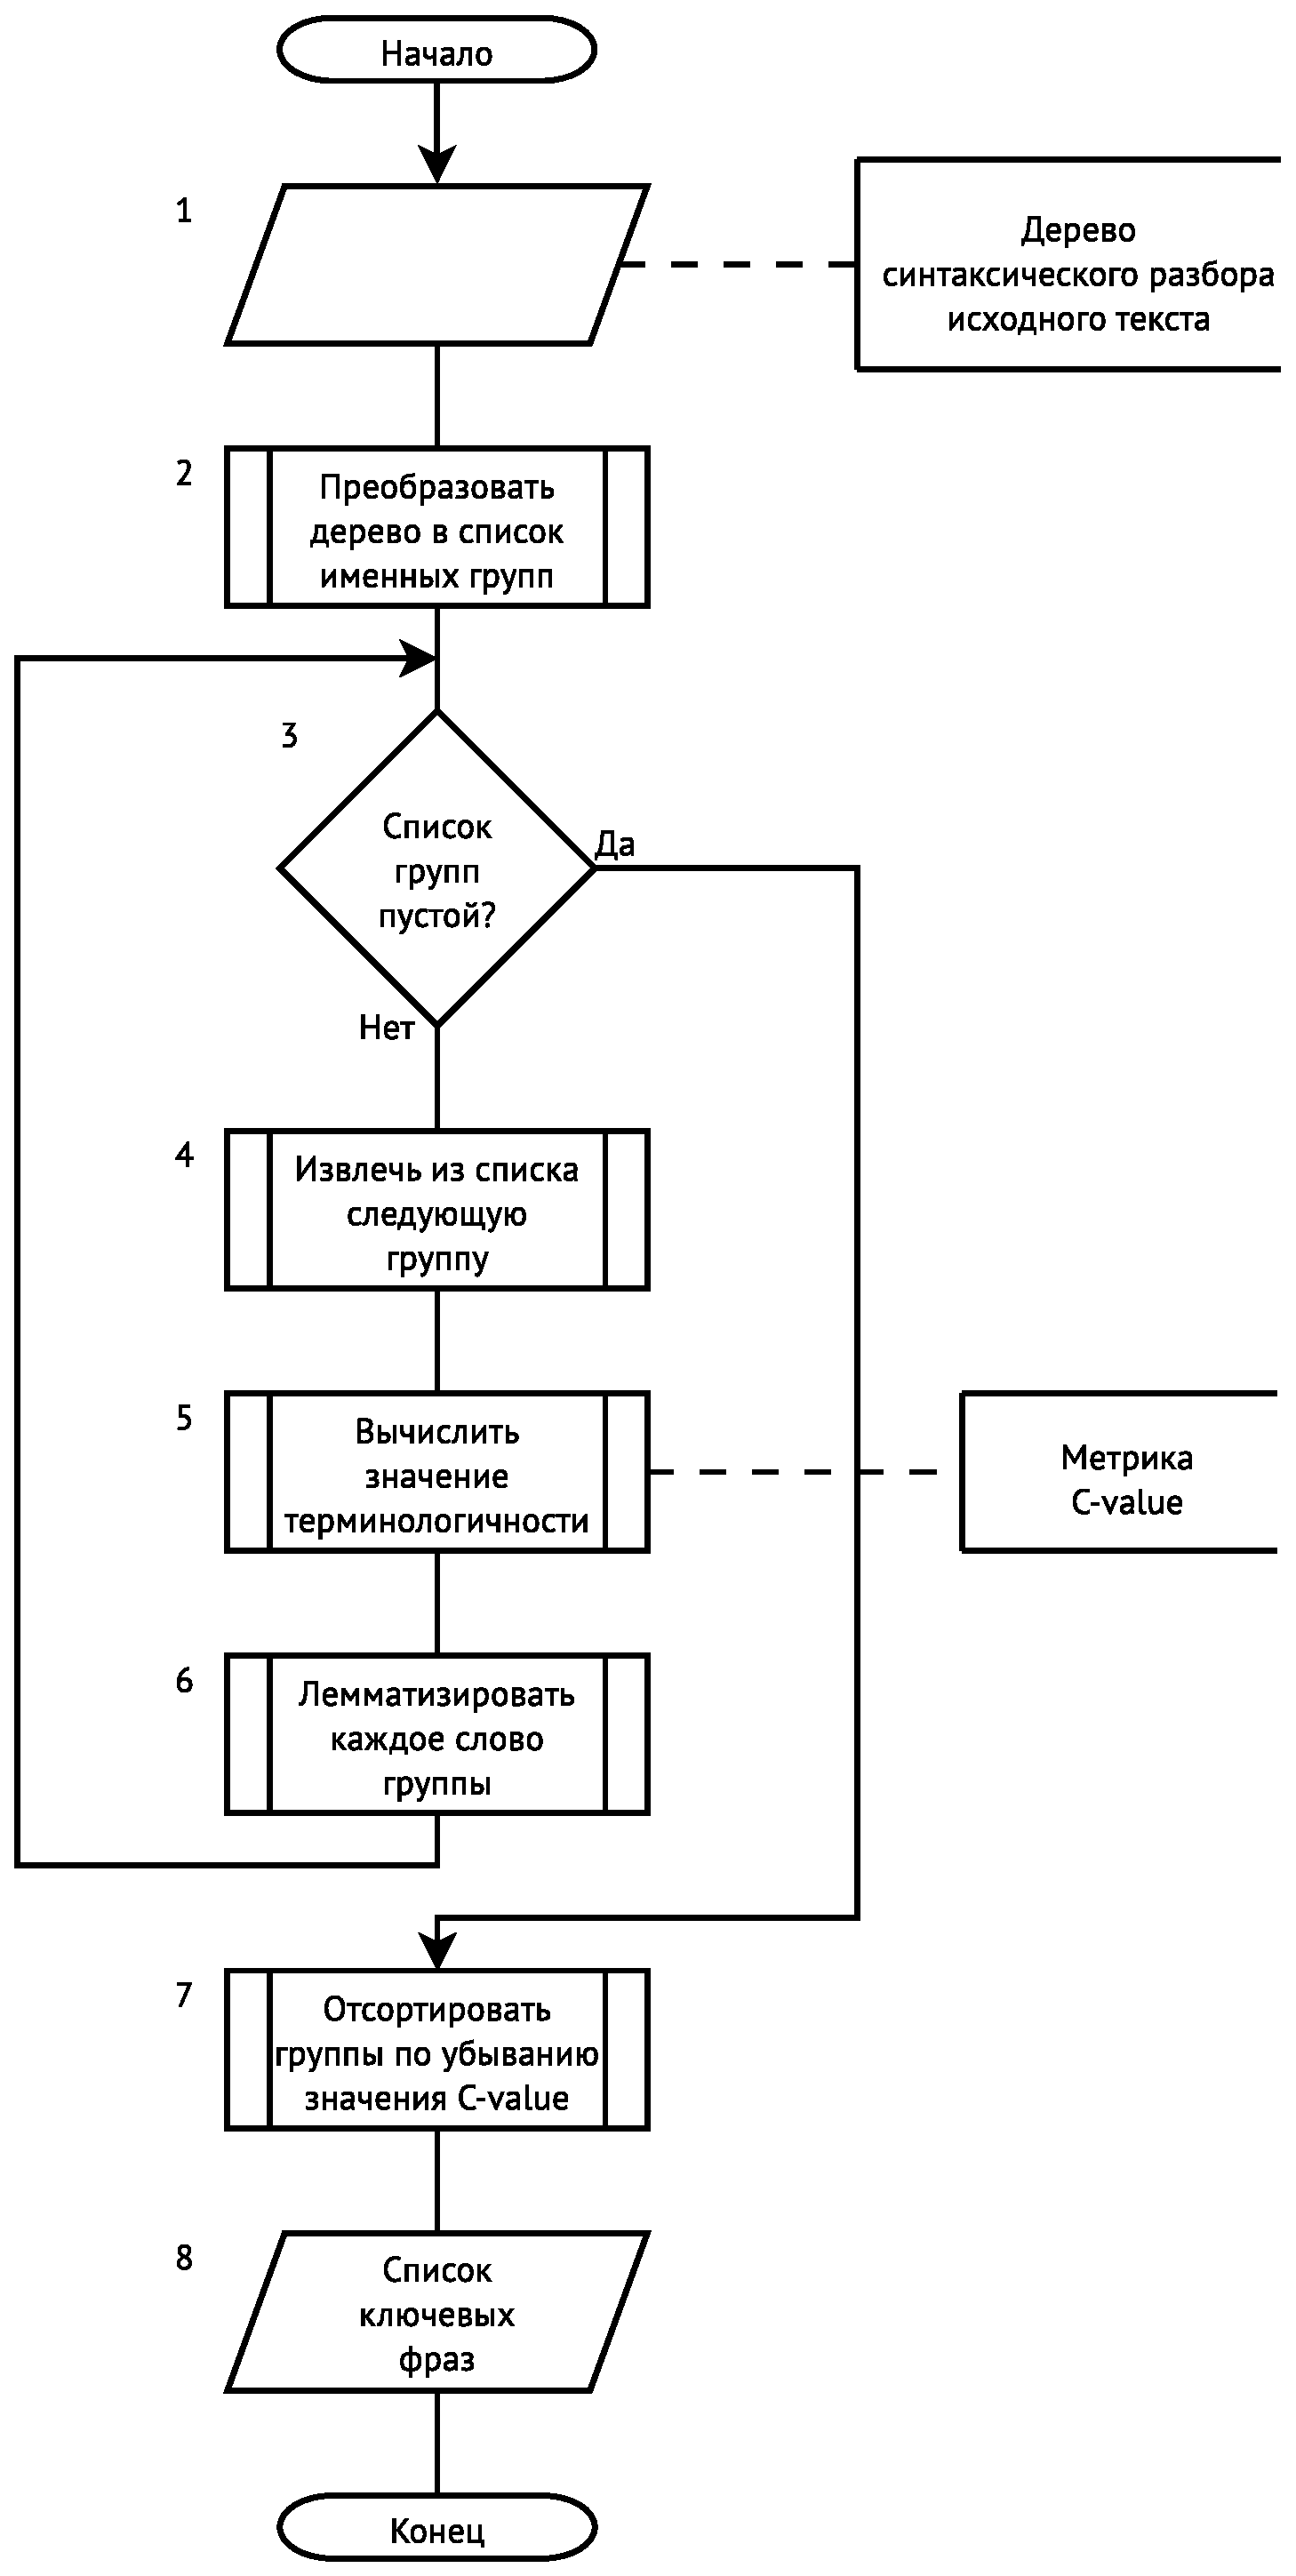
\includegraphics[scale=0.5]{Solution-Algorithm-Rank1a.eps}
  \caption{Алгоритмическая модель блока выделения ключевых фраз —
решения 1-го ранга}
  \label{fig:Solution-Algorithm-Rank1a}
\end{figure}

\subsubsection{Обзор морфологических анализаторов}
В качестве аналогов 1-го ранга по морфологическому анализу
рассмотрим морфологический анализатор АОТ и сравним его с
другими известными \cite{Lyashevskaya10} морфологическими
анализаторами:
\begin{itemize}
  \item mystem \cite{Mystem,Segalovich03}, разработчик —
компания «Яндекс»;
  \item Snowball \cite{Snowball,Porter93}, разработчик —
Dr.~M.~Porter;
  \item myaso \cite{Myaso}, разработчик — Д.~Усталов;
  \item pymorphy \cite{Pymorphy}, разработчик — М.~Коробов;
  \item TreeTagger \cite{TreeTagger,Schmid94}, разработчик —
H.~Schmid;
  \item TnT \cite{TnT,Brants00}, разработчик — T.~Brants.
\end{itemize}

В качестве критериев их сравнения выберем:
\begin{itemize}
  \item поддержка русского языка (``Р''):
  \begin{itemize}
    \item 0.0 — поддержка отсутствует;
    \item 1.0 — поддержка присутствует.
  \end{itemize}
  \item возможность определения части речи
(англ. \emph{POS-tagging}) и грамматических характеристик
слова (``Ч''):
  \begin{itemize}
    \item 0.0 — часть речи и морфологические шаблоны не
определяются;
    \item 0.5 — выполняется определение только части речи слова;
    \item 1.0 — определяется часть речи и грамматические
характеристики слова.
  \end{itemize}
  \item возможность выделения основы слова (англ.
\emph{stemming}) (``О''):
  \begin{itemize}
    \item 0.0 — основа слова не выделяется;
    \item 1.0 — основа слова выделяется.
  \end{itemize}
  \item качество анализа по итогам экспертной оценки (``К''):
  \begin{itemize}
    \item 0.0 — минимальная оценка;
    \item 1.0 — максимальная оценка.
  \end{itemize}
  \item доступность аналога (``Д''):
  \begin{itemize}
    \item 0.0 — использование аналога требует приобретения платной
лицензии или временной подписки;
    \item 0.5 — существуют полноценные бесплатные версии аналога,
$\beta$-версии или специальные версии для академических исследований;
    \item 1.0 — аналог распространяется как свободное программное
обеспечение.
  \end{itemize}
\end{itemize}

\begin{table}[H]
\caption{\label{tab:Analogs:Rank1}Сравнение существующих аналогов
1-го ранга по заданным критериям.}
\begin{tabular}{|c||c||*{5}{p{1cm}|}|c|}
\hline
  & Название   & \multicolumn{5}{c||}{Оценки по критериям} & \\
                \cline{3-7}
№ & аналога    &  Р  &  Ч  &  О  &  К  &  Д  & \huge $\Sigma$ \\
\hline
\hline
1 & АОТ        & 1.0 & 1.0 & 1.0 & 0.6 & 1.0 & 4.6 \\
\hline
2 & mystem     & 1.0 & 1.0 & 1.0 & 0.8 & 0.5 & 4.3 \\
\hline
3 & Snowball   & 1.0 & 0.0 & 1.0 & 0.6 & 1.0 & 3.6 \\
\hline
\textbf{4}
  & \textbf{myaso}
               & 1.0 & 1.0 & 1.0 & 0.7 & 1.0 & \textbf{4.7} \\
\hline
5 & pymorphy   & 1.0 & 1.0 & 1.0 & 0.5 & 1.0 & 4.5 \\
\hline
6 & TreeTagger & 1.0 & 1.0 & 1.0 & 0.7 & 0.5 & 4.2 \\
\hline
7 & TnT        & 1.0 & 1.0 & 0.0 & 0.7 & 0.5 & 3.2 \\
\hline
\end{tabular}
\end{table}

В результате сравнения аналогов (таблица~\ref{tab:Analogs:Rank1}),
целесообразно использовать аналог №4 (myaso, выделено жирным) в
качестве морфологического анализатора — готового решения
1-го ранга.

Структурная и алгоритмическая модели морфологического
анализатора (решения 1-го ранга) представлены на
рисунках~\ref{fig:Solution-Rank1b} и
\ref{fig:Solution-Algorithm-Rank1b}.

\begin{figure}[H]
  \centering
  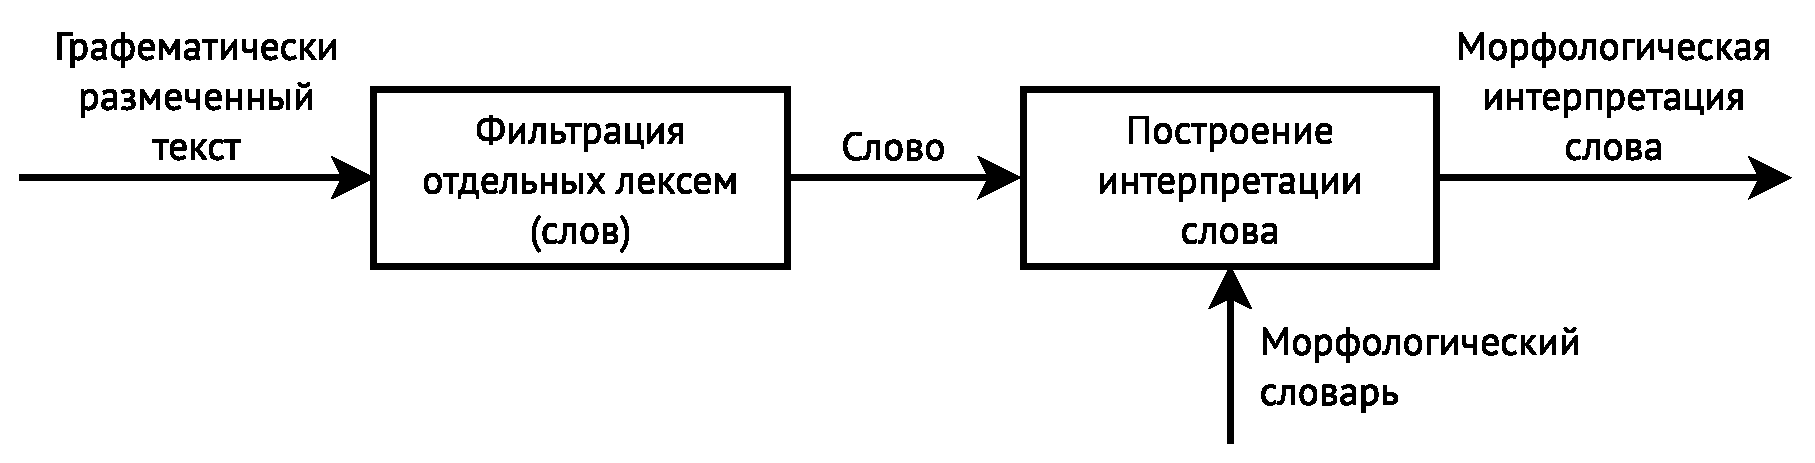
\includegraphics[scale=0.5]{Solution-Rank1b.eps}
  \caption{Структурная модель морфологического анализатора —
решения 1-го ранга}
  \label{fig:Solution-Rank1b}
\end{figure}

\begin{figure}[H]
  \centering
  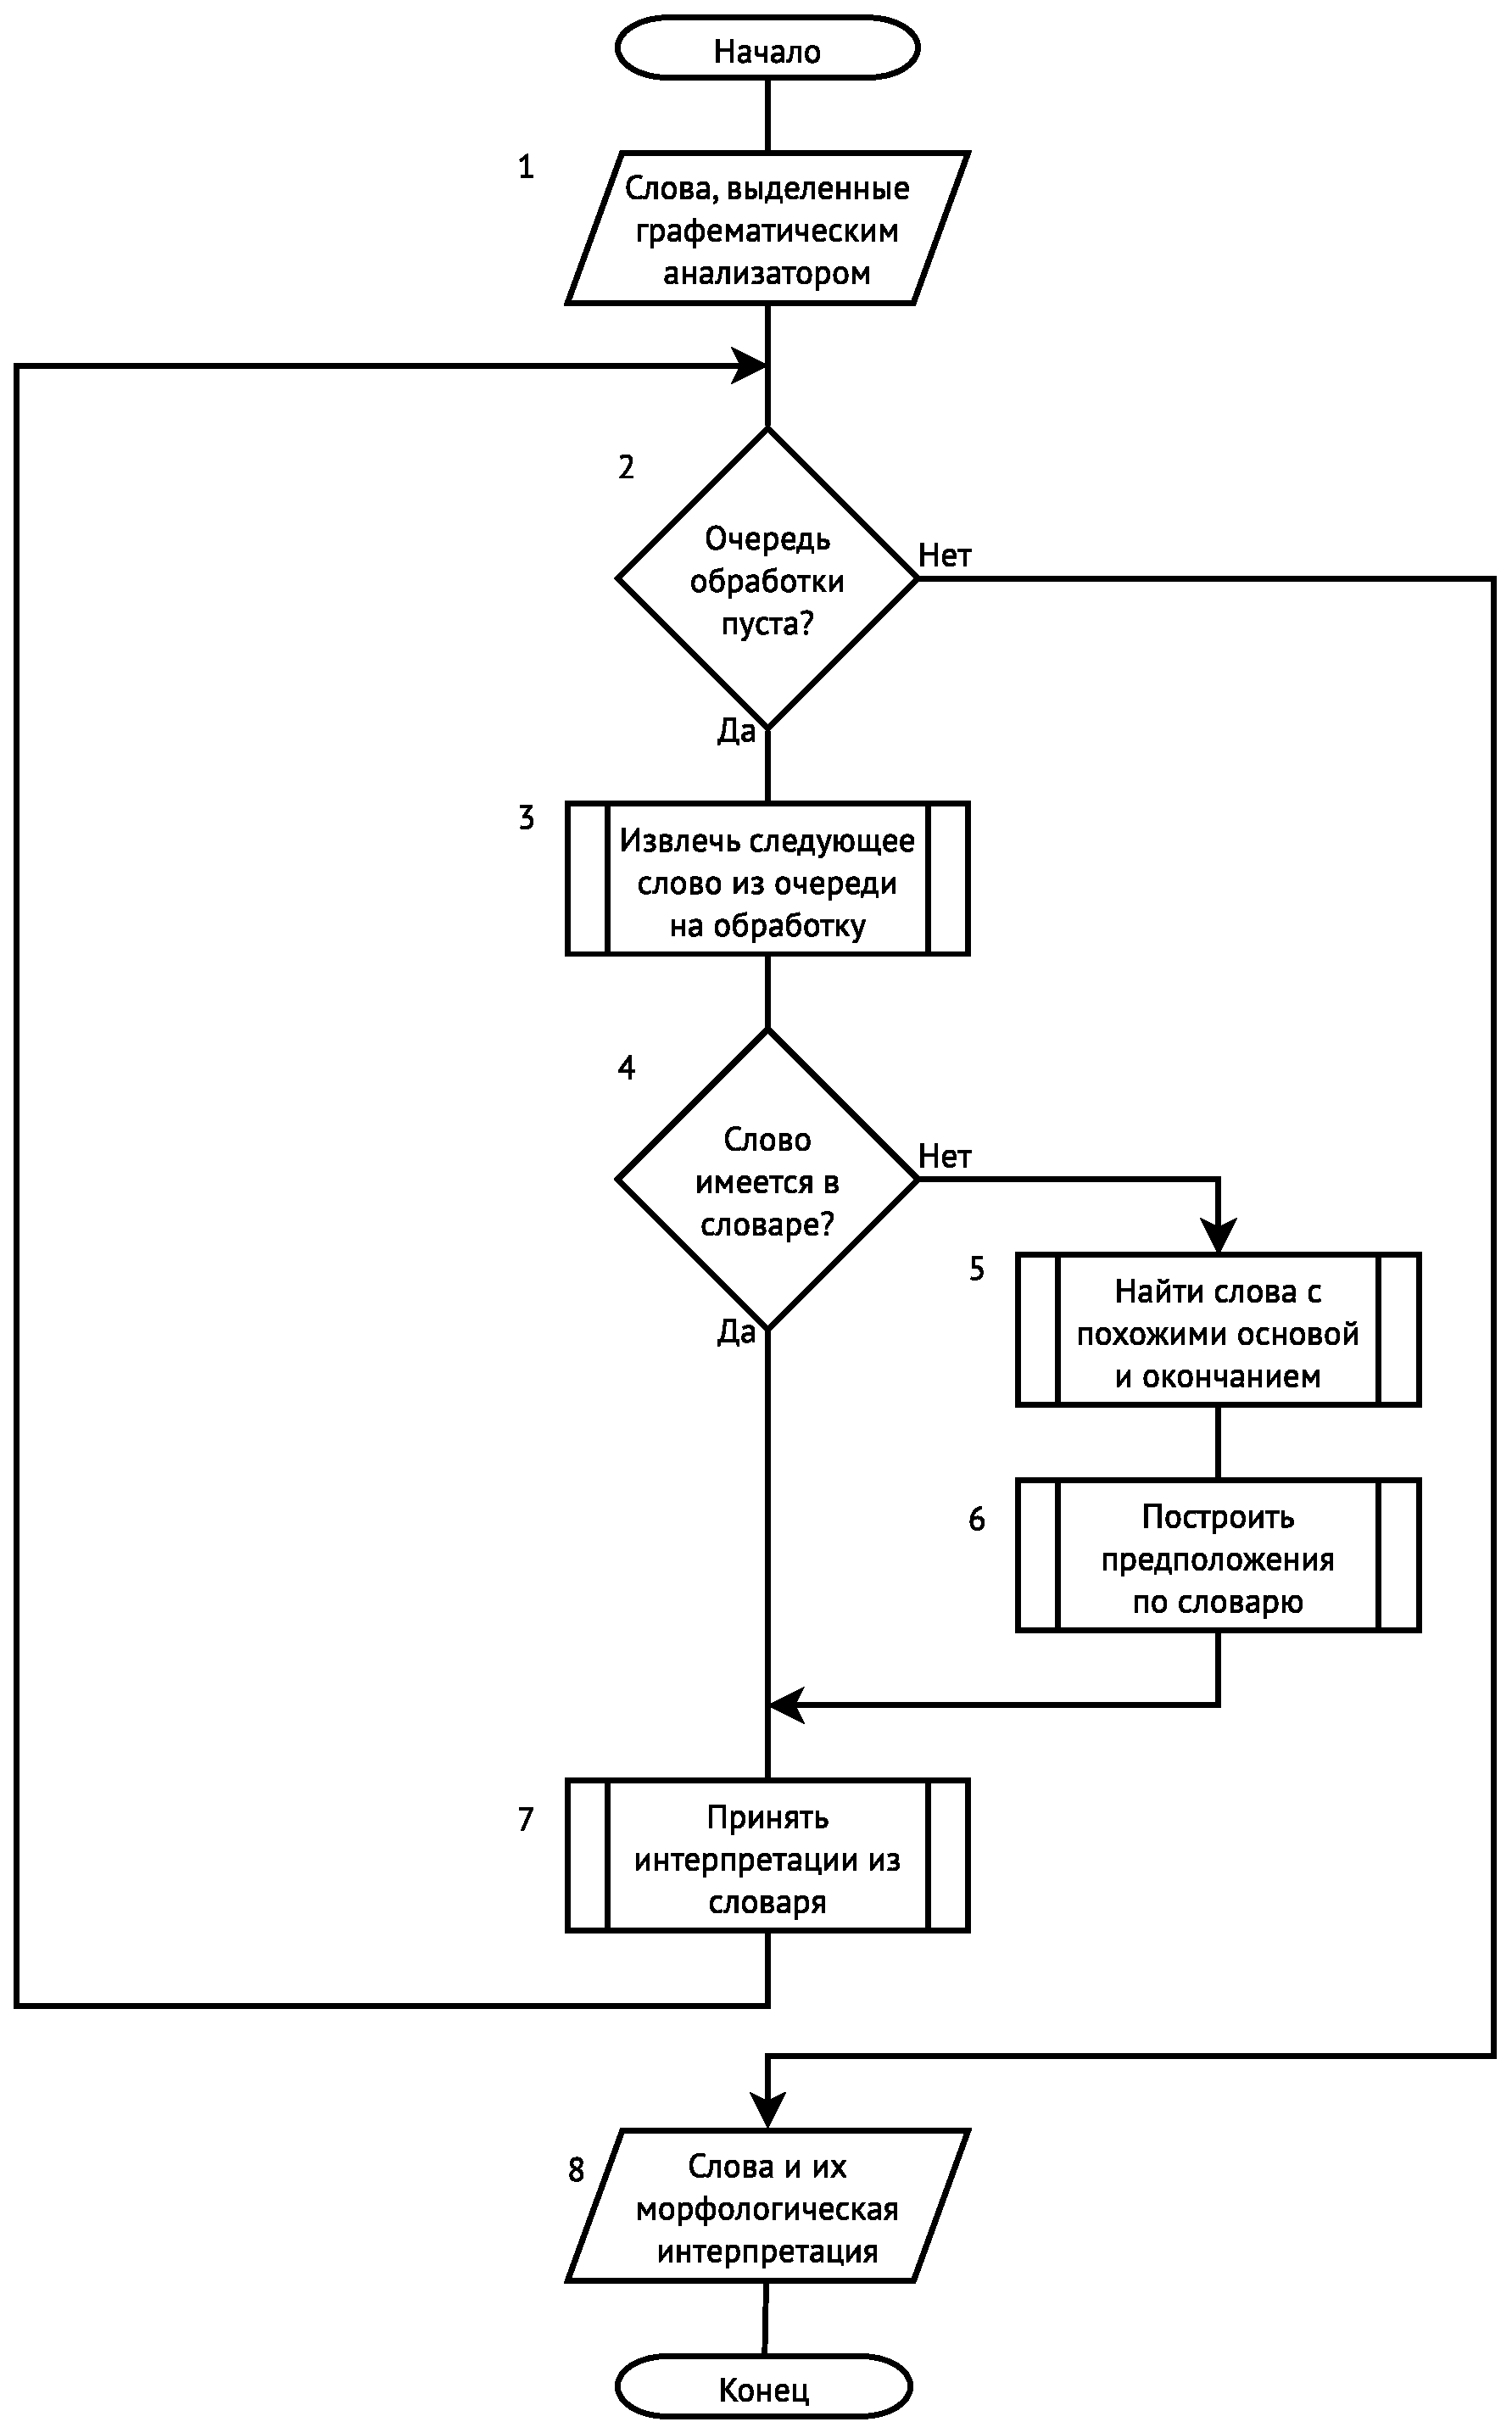
\includegraphics[scale=0.5]{Solution-Algorithm-Rank1b.eps}
  \caption{Алгоритмическая модель морфологического анализатора —
решения 1-го ранга}
  \label{fig:Solution-Algorithm-Rank1b}
\end{figure}

\section{Результаты и выводы}
В ходе выполнения литературно--аналитического обзора по теме
выпускной квалификационной работы:
\begin{itemize}
  \item приведена технология \ref{sec:Searching} поиска информации в
экспертных, электронных и библиографических источниках;
  \item на основе технологии поиска информации \ref{sec:Searching}
выбрано \totalbibs источников литературы по теме выпускной
квалификационной работы бакалавра;
  \item найдено 9 аналогов системы автоматического извлечения
ключевых фраз из текста на естественном языке;
  \item определён пакет эмпирических экспертных критериев
\ref{sec:Criteria} для оценивания найденных аналогов;
  \item составлена таблица~\ref{tab:Analogs} попарного сравнения
аналогов по критериям, обозначенным в \ref{sec:Criteria};
  \item на основе результатов сравнения аналогов
(таблица~\ref{tab:Analogs}) выбран прототип системы автоматического
извлечения ключевых фраз из текста на естественном языке;
  \item проведён критический анализ прототипа и предложены пути его
развития.
\end{itemize}
